\chapter{Background \label{ch:background}}
This chapter aims to give an introduction into the \acf{REXUS}/\acf{BEXUS} programme as a whole and the \acf{SETH} experiment as a part of this programme. Next the need for the \acf{ADS} is motivated and the measurement methods of the accelerometer and magnetometer explained.

\section{\acs{SETH} and the \acs{REXUS}/\acs{BEXUS} programme \label{sec:bg:seth_and_bx_programme}}

The \acs{REXUS}/\acs{BEXUS} programme is realised under a bilateral Agency Agreement between the \acf{DLR} and the \acf{SNSA}. The Swedish share of the payload has been made available to students from other European countries through a collaboration with the \acf{ESA}. EuroLaunch, a cooperation between the \acf{SSC} and the \acf{MORABA} of \acs{DLR}, is responsible for the campaign management and operations of the launch vehicles. Experts from \acs{DLR}, \acs{SSC}, \acs{ZARM} and \acs{ESA} provide technical support to the student teams throughout the project. \acs{REXUS} and \acs{BEXUS} are launched from \acs{SSC}, \acs{ESRANGE} Space Center in northern Sweden.


The first balloon of the \ac{REXUS}/\ac{BEXUS} programme, \textit{BEXUS 1}, launched on November 25$^{\mathrm{th}}$ 2002 at 15:53 UTC. Since then every year, except for 2003, 2020 and 2022, saw balloons being launched from the designated launch site \ac{ESRANGE} near the Swedish city of Kiruna \cite{IAC-08.E.1.1.4}\cite{bexus-campaign-history}.
The \ac{REXUS}/\ac{BEXUS} programme offers university student teams the opportunity to build their own experiment and have it fly on a stratospheric balloon. The programme spans around one year and is constructed as a scaled-down version of a real space mission. The \ac{SETH} takes part in the 16th \ac{BEXUS} cycle and is expected to fly between the 3$^\mathrm{rd}$ of October 2025 and 13$^\mathrm{th}$ of October 2025 from \ac{ESRANGE}.

The purpose of \ac{SETH} is to investigate the angular dependency of particle radiation in the upper atmosphere. To this end a means of measuring the experiments attitude and heading while on the gondola is required.

The main source of radiation in the atmosphere are \acp{GCR} that hit the earth isotropically from all directions. In 1935 Erich Regener and Georg Pfotzer published an article in \textit{Nature} presenting a figure (see fig. \ref{fig:regener1935}) which shows the radiation intensity measured by three Geiger-Müller Counters stacked on top of each other to have an aperture angle of about 20$^\circ$ around the zenith \cite{regener-pfotzer-1935}.

\begin{figure}[H]
    \centering
    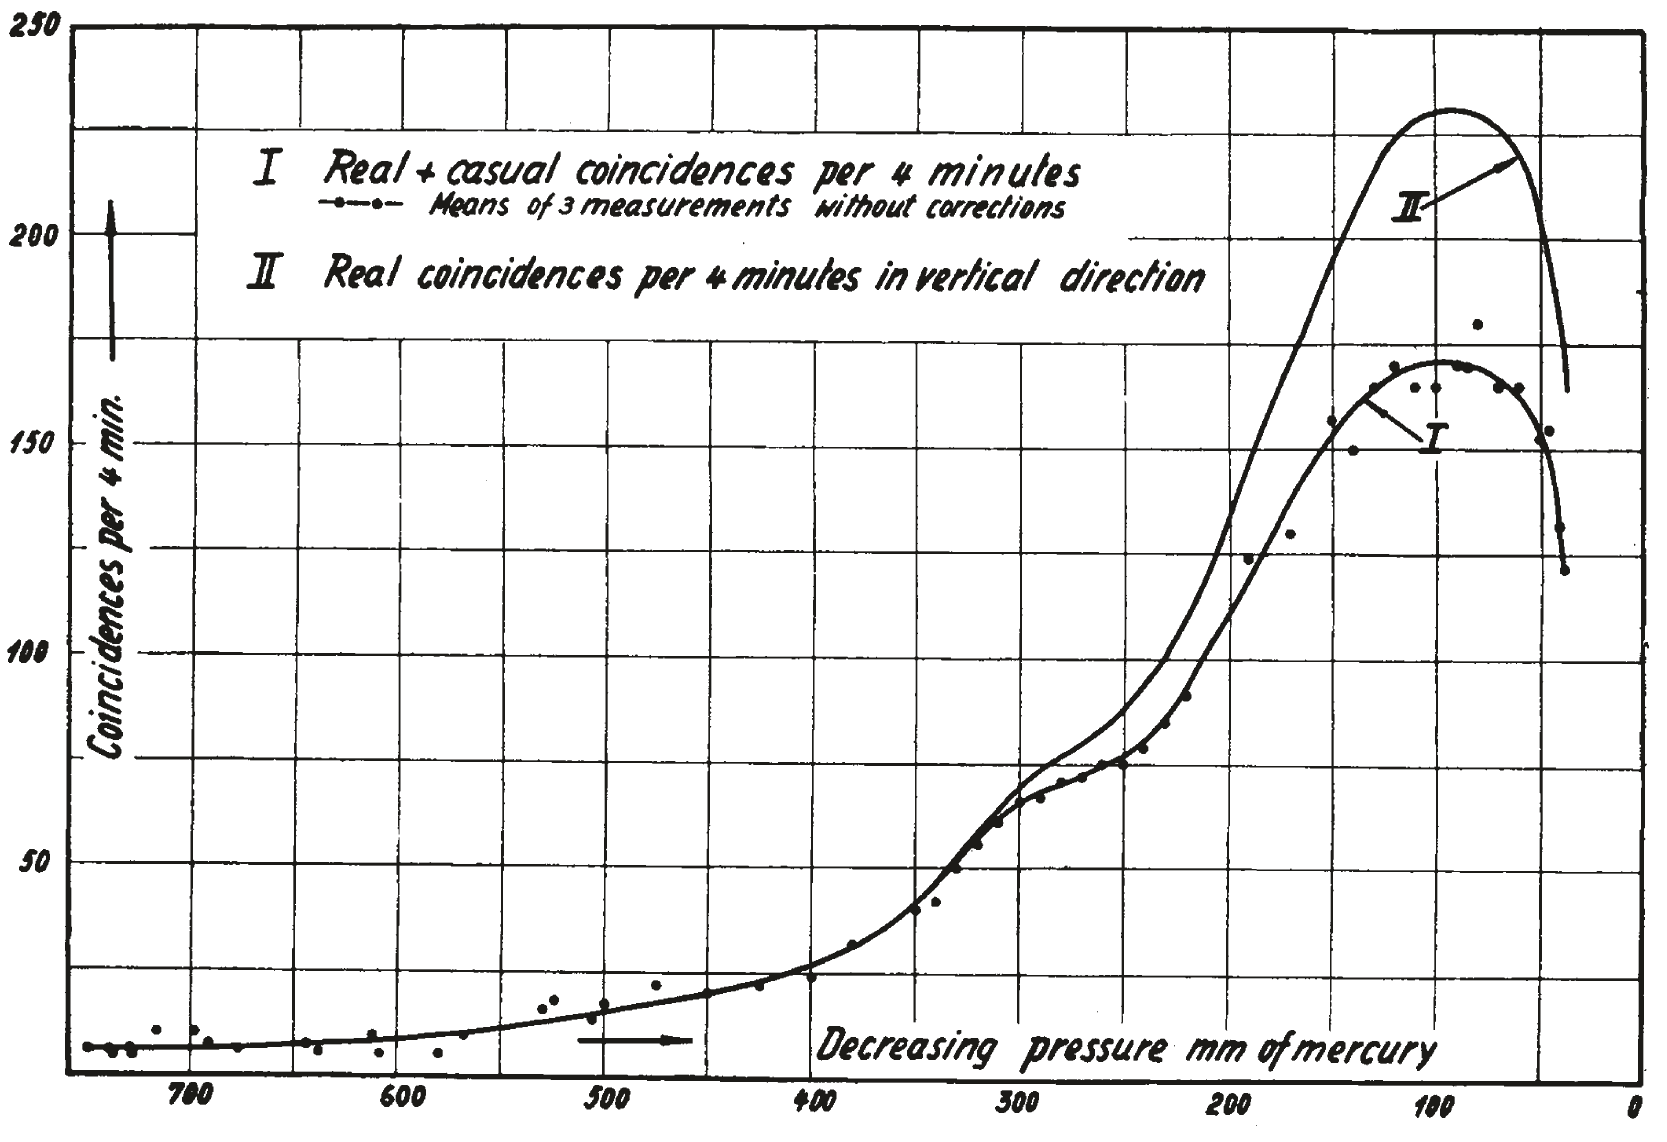
\includegraphics[width=0.8\linewidth]{images/01_background/original_regener_pfotzer.png}
    \caption[Regener-Pfotzer-Maximum as shown in \cite{regener-pfotzer-1935}]{Curve I shows the uncorrected coincidences per 4\,min. against ambient pressure in mm\ce{Hg}. Curve II shows the corrected coincidences taking the probability of coincidence counting against casual coincidences into account\cite{regener-pfotzer-1935}.}
    \label{fig:regener1935}
\end{figure}

Eighty Years later, the \ac{ADAM} \ac{BEXUS} Team around Dennis Trautwein showed that the fluence of particles for a given altitude varied with the zenith angle. Figure \ref{fig:martensen2015} taken from \cite{martensen2015} shows the angular distribution of particle fluence at an altitude of 27\,km.

\begin{figure}[H]
    \centering
    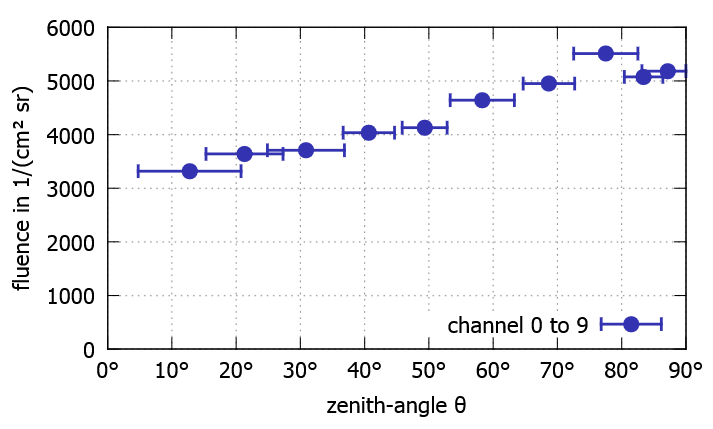
\includegraphics[width=0.6\linewidth]{images/01_background/martensen.png}
    \caption[Results of \acs{ADAM} at 27\,km]{Angular distribution of the charged particle fluence at an altitude of 27\,km \cite{martensen2015}.}
    \label{fig:martensen2015}
\end{figure}

Counting rate $C$ (coincidences per unit time) and isotropic Intensity $I_0$ (Fluence per unit time) share a linear relationship with the Geometrical Factor $G$ as coefficient, as is given in eq. \eqref{eq:sullivan}\cite{SULLIVAN19715}.
\begin{equation}
    C=G\cdot I_0
    \label{eq:sullivan}
\end{equation}

\newpage
The \ac{SETH} experiment has multiple well defined goals:

    \underline{\textbf{Primary Objectives}}
		\begin{description}\setlength\itemsep{-1em}
			\item[Obj. 1.1:] To measure Primary Galactic Cosmic Rays and secondary particles around the Regener-Pfotzer maximum and analyse its angular dependency. (Scientific)
			\item[Obj. 1.2:] To test a new electronics design featuring 48 signal channels. (Technical)
		\end{description}
	\underline{\textbf{Secondary Objectives}}
		\begin{description}\setlength\itemsep{-1em}
			\item[Obj. 2.1:] To measure the different particle species of Primary Galactic Cosmic Rays. (Scientific)
            \item[Obj. 2.2:] To measure showering of a very high energy electron in the \ac{BGO} detectors. (Scientific)
            \item[Obj. 2.3:] To measure the cardinal direction of the gondola. (Technical)
		\end{description}

The goals of \ac{SETH} which are the motivation for this thesis are Objectives 1.1 and 2.3: to measure the angular distribution of the Regener-Pfotzer-Maximum in the zenith and in the azimuthal angle and the determination of the gondolas cardinal direction (i.e. heading). A \ac{CAD} model of parts of the \ac{SETH} detector is shown in fig. \ref{fig:seth_cad}. The zenith and azimuthal angle of an incoming particle can be determined through the coincidence of two photodiodes (active area shown in orange).

\begin{figure}[H]
    \centering
    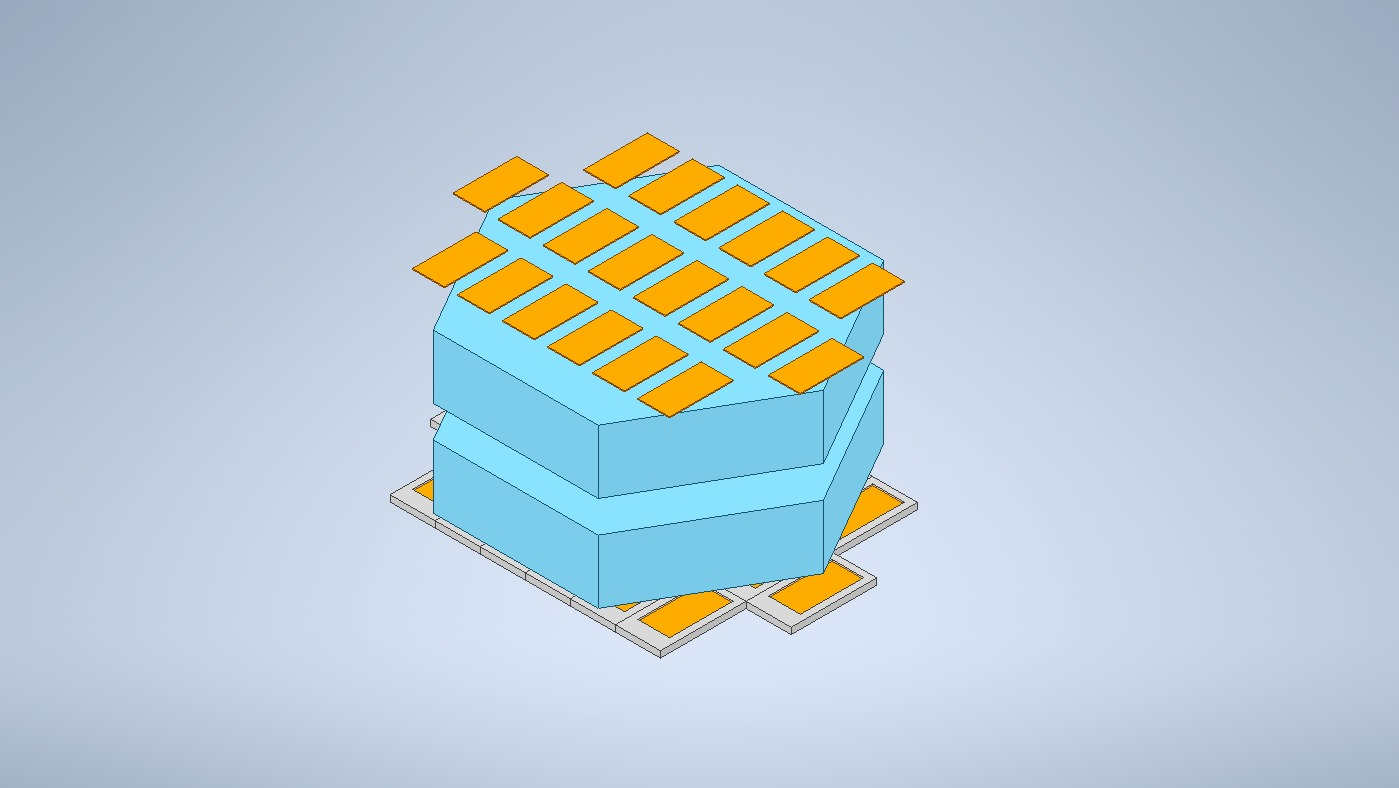
\includegraphics[width=0.5\linewidth, trim = {5cm 0cm 5cm 0cm}, clip]{images/01_background/SETH-Sketch.jpeg}
    \caption[\ac{SETH} detector sketch]{\ac{CAD} model of the \ac{SETH} detector showing the array of diodes.}
    \label{fig:seth_cad}
\end{figure}

The gondola hanging from the \ac{BEXUS} balloon does not have a fixed orientation in space. The wind will incite the gondola to rotate and swing during all phases of flight. Thus to get a reliable measurement of the angular distribution of the Regener-Pfotzer-Maximum in the azimuth domain, accurate heading information is required so as to know which direction particles travelling through the telescope hail from. The heading may occasionally be called yaw or azimuth.

\framebox[\linewidth][c]{\textbf{Objective 1.: The gondolas heading shall be measured.}}

As mentioned above, the gondola will also experience swinging or more accurately pitching and rolling. This is a deflection from the plane parallel to the local earths surface, split into the lateral and longitudinal axis of the gondola (for comparison see fig. \ref{fig:attitude}). As the gondola is a rigid body and all experiments are fixated, the attitude of the gondola as a whole is the same as the attitude of our experiment.

\framebox[\linewidth][c]{\textbf{Objective 2.: The gondolas attitude shall be measured.}}

\begin{figure}[H]
    \centering
    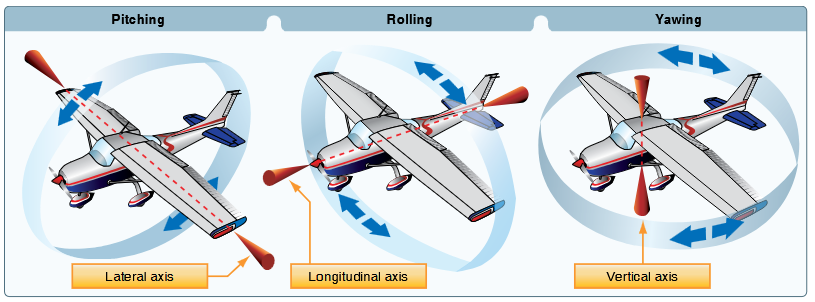
\includegraphics[width=0.5\linewidth]{images/01_background/axes_of_an_airplane.png}
    \caption[Axes of an airplane]{Axes of an airplane, from \cite{pilot-handbook}.}
    \label{fig:attitude}
\end{figure}

It is the job of the \ac{ADS} to fulfil objectives 1 and 2. This thesis will cover the implementation, calibration and preliminary testing of the \ac{ADS}.

\section{Sensing Elements \label{sec:bg:sensing_elements}}
There are many different methods of measuring magnetic fields and accelerations as presented in \cite{}, \cite{} or \cite{}. This chapter will introduce the methods that are utilised by the sensors chosen for the \ac{ADS}.

\subsection{Magnetometer \label{sec:bg:magnetometers}}
To fulfil Objective 1, which is to determine the gondola's heading, a magnetometer is used. The 3-axis magnetometer will allow us to determine magnetic north and with the \ac{WMMHR} the local declination (i.e. the deviation from true north) can be calculated resulting in the gondolas true heading. 

The sensing technology of the chosen sensor is not mentioned in any official documentation. The only acknowledgement of \ac{STM} to the various questions posted on their community site is a short reply\footnote{\url{https://community.st.com/t5/mems-sensors/does-anyone-know-what-s-the-sensing-technology-about-lis3mdl/m-p/111961}} by Eleon Borlini\footnote{\url{https://www.linkedin.com/in/eleon-borlini-5520b477/}}, "Product development manager - Head of validation methodology" at \ac{STM}. In this post he states that it is a \ac{TMR} sensor with no further elaboration or prove. Thus we are forced to believe them as determining the sensing technology is out of the scope of this thesis.

First published in \cite{JULLIERE1975} in 1975, the tunnelling of electrons between (ferro-)magnetic films is the basis for many modern sensors used to determine the magnitude and direction of a magnetic field. It is expected that in the future \ac{TMR} sensors will become the most popular solution in magnetic sensing applications \cite{yan2022}.

A \ac{MTJ} is built from two ferromagnetic materials with an electrical insulator in between. The external magnetic field which is to be measured can then be characterised by the electrical resistance of the junction. The magnetization $\vec{M}=\frac1V\sum_V\vec{p}_m$ of each of the two ferromagnets is the magnetic moment per unit volume \cite{Demtröder2017-eo}. It is influenced by the field $\vec{B}$, aligning the magnetization $\vec{M}$ with the external field in accordance with the magnetic field strength $
|\vec{B}|$. The proportionality between magnetization and applied field strength is given by $\chi/\mu\mu_0$ with the magnetic susceptibility $\chi$, relative permeability $\mu$ and $\mu_0$ vacuum magnetic permeability.\\
In both magnets there are electrons parallel and antiparallel to the magnetization axis. Given below in eqs. \eqref{eq:bg:parallel_conductance} and \eqref{eq:bg:antiparallel_conductance} is the resistance of the \ac{MTJ} according to \cite{JULLIERE1975}. The indices ($\uparrow\uparrow$) and ($\uparrow\downarrow$) signalise a parallel and antiparallel spin of the tunnelling electrons, relative to the magnetization. The $a$ and $a'$ denote the fraction of all tunnelling electrons with parallel or antiparallel spin.
\begin{align}
    R_{\uparrow\uparrow}\propto \frac{1}{a^{}_{\uparrow\uparrow}a'_{\uparrow\uparrow}+a^{}_{\uparrow\downarrow}a_{\uparrow\downarrow}'}
    \label{eq:bg:parallel_conductance} \\
     R_{\uparrow\downarrow}\propto \frac{1}{a^{}_{\uparrow\uparrow}a'_{\uparrow\downarrow}+a^{}_{\uparrow\downarrow}a'_{\uparrow\uparrow}}
     \label{eq:bg:antiparallel_conductance}
\end{align}

The relative resistance change then becomes \eqref{eq:bg:rel_res} according to \cite{moodera1995}.
\begin{equation}
    \frac{\Delta R}{R}=\frac{R_{\uparrow\downarrow} - R_{\uparrow\uparrow}}{R_{\uparrow\downarrow}}
    \label{eq:bg:rel_res}
\end{equation}

The sensor utilises this measurable change in resistance to determine the strength of the external field. Multiple ways to linearise the \ac{MTJ} response, e.g. , are utilised as presented in \cite{yan2022}.

\subsection{Accelerometer \label{sec:bg:accelerometers}}
To fulfil the second objective an accelerometer is used. The sensing element is a type of \ac{MEMS}: A silicon structure, called a proof mass, anchored to a substrate but able to move freely in at least 1 direction. On the proof mass there are small electrodes pointing outward that form a plate capacitor with static plates on the substrate (or handle layer), as shown in fig. \ref{fig:bg:mems_accelerometer}. The formula for the capacitance $C$ of a plate capacitor with area $A$ is given in eq. \eqref{eq:bg:cad}. The capacitance is inversely proportion la to the distance $d$ of the plates.
\begin{equation}
    C=\frac{A}{d}
    \label{eq:bg:cad}
\end{equation}

\begin{figure}[H]
    \centering
    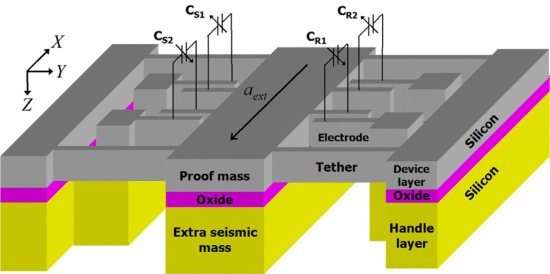
\includegraphics[width=\linewidth]{images/01_background/mems_acc_diagram.png}
    \caption{Schematic representation of a \ac{MEMS} accelerometer taken from \cite{abdolvand2007}}
    \label{fig:bg:mems_accelerometer}
\end{figure}

When an acceleration $\vec{a}_{\mathrm{ext}}$ is applied to the proof mass, it displaces from its initial position and the capacitance in the capacitors changes. Figure \ref{fig:bg:mems_accelerometer} is only one possible way of realizing the sensor. Other accelerometers may also have external electrodes on both sides of the proof mass' electrodes simultaneously measuring an increase and a decrease. 


\section{Measurement Errors \label{sec:bg:measurement_errors}}
The sensing elements described in sections \ref{sec:bg:magnetometers} and \ref{sec:bg:accelerometers} each work in one dimension. To get a three-axis sensor, three sensing elements are assembled orthogonally to one another. In this automated process, errors in the alignment of the three sensing elements may occur. We will interpret the misalignment of the three sensing axes of a sensor as a $3\times3$ matrix $C_{m}$ \cite{magcal}\cite{non-orthonogality}.

Due to mechanical stresses, unshielded magnetic fields, or other influences during production of the sensing elements they each may have a scale factor different from 1. This means when a field of magnitude 1 is applied the sensor may read 1.1, and 0.55 when a field of magnitude 0.5 is applied. In this case, the scale factor would be 1.1. As each sensing element may have experienced different conditions during production, we will consider one scale factor per axis, resulting in a $3\times1$ matrix $C_{sf}$.

The third error intrinsic to all 3-axis sensors is a zero bias, or null shift. This error may again have its origin during production of each sensing element and affects each axis differently. This error quantifies the offset, that the scaled measured value has from its true value. For example if no field is applied but the sensor reads a magnitude of 0.5 then that is the null shift. For the sensor as a whole, this is another $3\times1$ matrix $C_{zb}$.

While the errors introduced above are present in accelerometers and magnetometers alike the latter suffers from two more errors. These are soft iron and hard iron errors which are a natural part of the measurement of magnetic fields.\\
The hard iron errors $\delta\vec{B}$ are interfering magnetic fields from sources of constant magnetic fields around the sensor. Examples may be iron screws, nuts, or washers. This is a $3\times1$ matrix.

The last error to be discussed is a $3\times3$ soft iron error matrix $C_{si}$.

The measured quantities, denoted by the subscript "meas", can thus be expressed by the true vector fields as shown below. The superscripts $g$ and $B$ denote the accelerometer and magnetometer respectively.
\begin{align}
    \vec{G}_{meas}&=C^g_mC^g_{sf}\vec G+C_{zb}^g \label{eq:bg:g_with_errors}\\
    \vec{B}_{meas}&=C^B_mC^B_{sf}C^B_{si}(\vec{B}+\delta\vec{B})+C_{zb}^B
    \label{eq:bg:b_with_errors}
\end{align}

To simplify these equations, the misalignment of the sensors is assumed as negligible. The misalignment matrix for this case is shown in eq. \eqref{eq:bg:misalignment_matrix}. That this assumption is justified is shown in sec. \ref{sec:da:misalignment}.
\begin{equation}
    C_m= \begin{pmatrix} 1 & 0 & 0 \\
                         0 & 1 & 0 \\
                         0 & 0 & 1 \end{pmatrix}
                         \label{eq:bg:misalignment_matrix}
\end{equation}